

%%%%%%%%%%%%%%%%%%%%%%%%%%%%%%%%%%%%%%%%%%%%%%%%%%%%%%%%%%%%
%%%%%%%%%%%%%%%%%%%%%%%%%%%%%%%%%%%%%%%%%%%%%%%%%%%%%%%%%%%%%
%
%  %%%%%%%  %    %  %%%%%%  %%%%%%  %%%%%%%  %%%%%%%  %%%%%
%  %        %    %  %    %  %     %    %     %        %    %
%  %        %    %  %%%%%%  %     %    %     %        %    %
%  %        %%%%%%  %    %  %%%%%%     %     %%%%%    %%%%%
%  %        %    %  %    %  %          %     %        %    %
%  %%%%%%%  %    %  %    %  %          %     %%%%%%%  %     %
%
%%%%%%%%%%%%%%%%%%%%%%%%%%%%%%%%%%%%%%%%%%%%%%%%%%%%%%%%%%%%%
%%%%%%%%%%%%%%%%%%%%%%%%%%%%%%%%%%%%%%%%%%%%%%%%%%%%%%%%%%%%%
\chapter{Topological Data Analysis}
\label{sec:barcodes}

% \dictum[Plato's Phaedrus 265e, translated by R. Hackforth]{``We are enabled to divide into forms, following the objective articulation; we are not to hack off parts like a clumsy butcher.''}

\begin{quote}
{\em``We are enabled to divide into forms, following the objective articulation; we are not to hack off parts like a clumsy butcher.''}
\begin{flushright} --- Plato's Phaedrus 265e, translated by R. Hackforth \end{flushright}
\end{quote}

Suppose two patients enter an office with a recent diagnosis of cancer. If they are very lucky, they might have their respective tumors biopsied and sent off for genetic analysis. The genetic analysis consists of measuring the gene expression levels of over a thousand genes in each of the respective tumors. These two sets of expression levels are then compared with a few hundred other tumor samples, where varying therapies were used to varying degrees of success. How should the doctor determine which course of action to take? If we are to carve the universe at its joints, on which side do these patients lie?

A similar, but apparently less dramatic, situation occurs in topology. Given two topological spaces $X$ and $Y$, how do we discern whether $X$ and $Y$ are essentially the same or different? The entire apparatus of algebraic topology was developed to address this problem. It turns out that these two situations are not just formally similar. Topological data analysis stems from the observation that data of the above form can give rise to topological spaces, which can in turn be discriminated using classical constructions such as homology~\cite{lum2013extracting}.

\section{Point Clouds and Persistent Homology}
\label{subsec:pointclouds}\index{point cloud}\index{persistent homology}

To illustrate why the applicability of homological methods is not so far-fetched, consider the following toy problem, which serves as the standard entr\'ee into \textbf{persistent homology}.
\begin{figure}[ht]
	\centering
	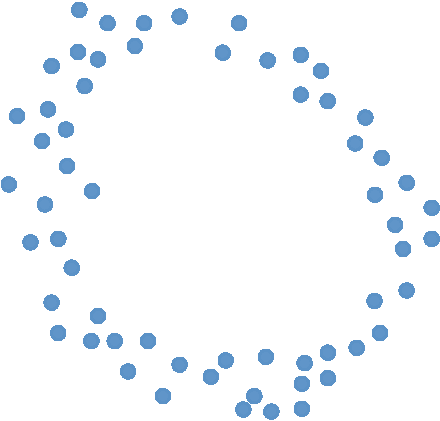
\includegraphics[width=.7\textwidth]{point_cloud.pdf}
	\caption{Point Cloud Data}
	\label{fig:point_cloud_data}
\end{figure}
Consider a finite set of points $\{x_i\}\subset \R^n$. How do we describe the perceived shape of such a set of points, such as the set depicted in Figure \ref{fig:point_cloud_data}? The human brain is a pattern-making machine that connects the dots and returns the knee-jerk response that the points in Figure \ref{fig:point_cloud_data} appears to form a circle. However, what do we mean by this and how can we automate this process so as to remove human subjectivity? 

Mathematics abounds with rigorous formulations of what does or does not look like a circle. However, only topology provides a definition that is robust with respect to perturbation and noise. One universal definition of a circle is given by the Eilenberg-Mac Lane space $K(\Z,1)$, which is homotopy equivalent to $S^1$. However, homology provides a shape descriptor based on linear algebra, which can be efficiently computed. But there is still the problem that the homology of the set of points in Figure \ref{fig:point_cloud_data} is not isomorphic to the homology of the circle. To get around this, we consider the union of Euclidean balls of some radius $r$ $\cup B(x_i,r)=:X_r$, which mirrors the ``connecting the dots'' procedure that the brain applies. Then one observes that there are natural inclusions
\[
	X_{r_0}\hookrightarrow X_{r_1} \hookrightarrow X_{r_2} \hookrightarrow X_{r_3} \cdots
\]
whenever $r_0\leq r_1\leq r_2 \leq \cdots$ and so on. Applying the $i$th homology functor $H_i(-;k)$ turns this diagram of spaces into a diagram of vector spaces, which defines a persistence module, cf. Definition \ref{defn:persistence_module}.
\begin{equation*}
%\label{eq:persist}
	H_i(X_{r_0};k) \to H_i(X_{r_1};k) \to H_i(X_{r_2};k) \to H_i(X_{r_3};k) \to \cdots 
\end{equation*}
By applying the structure theorem~\ref{thm:crawleyboevey}, we can determine the barcodes of the collection of points. Long bars are considered to be robust topological signals in the data set. For Figure \ref{fig:point_cloud_data}, there would be one long bar in the persistence module corresponding to $H_0$, indicating that after a certain radius the the space $X_r$ is connected, and another long bar in the module corresponding to $H_1$, indicating the apparent circle in the data set. 

To summarize, we have the following prototypical pipeline of topological data analysis.
\begin{defn}[Point Cloud Persistence]\label{defn:point-cloud-persistence}\index{persistent homology!sublevel set}
The \textbf{point cloud persistence pipeline} consists of the following ingredients and operations:
\begin{enumerate}
\item Let $X$ denote a point cloud, i.e. the union of a finite set of points $\{x_i\}\subset \R^n$.
\item The union of balls $X_r:=\cup_{x_i\in X} B(x,r)$ (or the Vietoris-Rips complex~\cite{ghrist-barcodes}) defines a functor from the real line, viewed as poset, to the category of topological spaces (simplicial complexes) and maps, i.e. 
\[
G:(\R,\leq)\to\Top \qquad r \rightsquigarrow X_r \qquad r\leq r' \rightsquigarrow X_r\hookrightarrow X_{r'}
\]
\item Postcomposing this functor with homology $H_{\ast}$, defines a graded representation of the real line, which is equivalently a graded sheaf on the Alexandrov topology or a graded persistence module:
\begin{equation*}
%\label{eq:persist}
	H_{\ast}(X_{r_0};k) \to H_{\ast}(X_{r_1};k) \to H_{\ast}(X_{r_2};k) \to H_{\ast}(X_{r_3};k) \to \cdots 
\end{equation*}
\item Applying Theorem \ref{thm:crawleyboevey} produces a Remak decomposition of this representation into a multiset of interval modules, which is visualized as a barcode by the end user. 
\end{enumerate}
\end{defn}

The first and second steps in this pipeline offer the chance for endless modification and application. Instead of considering a collection of points, one can start with a space $X$ and a function $f:X\to\R$ and consider the family of sub-level sets $X_r:=f^{-1}(-\infty,r]$. As long as the function and space are sufficiently nice, we can use Theorem \ref{thm:crawleyboevey} to produce a barcode.

\begin{exr}
Determine the barcodes associated to the function $f(x)=x^3-x$.
\end{exr}

\begin{exr}
Recast the basic theorems of Morse theory in terms of barcodes. See Figure \ref{fig:persistence_torus} for inspiration.
\end{exr}

\subsection{Level Set and Zigzag Persistence}


Despite their successes, persistence modules are not the end-all, be-all of topological data analysis. In~\cite{zigzag} Gunnar Carlsson and Vin de Silva gave three examples where diagrams of vector spaces and maps of the form
\[
	V_1 \leftrightarrow V_2 \leftrightarrow V_3 \leftrightarrow  \cdots \leftrightarrow V_{n-2} \leftrightarrow V_{n-1} \leftrightarrow V_n
\]
are of interest. One example comes from estimating the probability density function from which a point-cloud is drawn. One can try to smooth the data by defining a function $\rho_r(x)$ that counts the number of points within a radius $r$ of the point $x$. If one then tries to take the 25\% densest points measured according to a sequence of radii $r_1<r_2<\cdots <r_n$, the the only way of comparing features comes from a \textbf{zigzag} diagram of the form
\[
X_{r_1}^p \rightarrow X_{r_1}^p\cup X_{r_2}^p \leftarrow X_{r_2}^p \rightarrow \cdots \leftarrow X_{r_n}^p  
\]
where $X^p_{r_k}$ indicates the $p\%$ densest points measured according to the function $\rho_{r_k}(x)$. Similarly, if one has a function $f:X\to\R$, but not the computational power to investigate the entire sub-level set $f^{-1}(-\infty,r]$, one could choose a mesh $t_0<t_1<t_2<\cdots <t_n$ and consider the zigzag of pre-images given by
\[
f^{-1}(t_0)\rightarrow f^{-1}[t_0,t_1]\leftarrow f^{-1}(t_1) \rightarrow \cdots \leftarrow f^{-1}(t_n).
\]
Applying homology in some degree $i$ gives the traditional definition of \textbf{level set persistent} homology. This complicates the usual TDA pipeline because, a priori, the structure theorem \ref{thm:crawleyboevey} fails to apply. Fortunately, Gabriel's Theorem \ref{thm:gabriel} tells us that the direction of the arrows doesn't matter for the representations of $A_n$ type quivers, so the decomposition into interval modules still applies; we still have barcodes~\cite{zigzag}.

The fully general definition of level set persistence usually given adheres to this perspective that the assignment of homology to closed intervals is fundamental.
\begin{defn}\index{category!of intervals}
The \textbf{interval category} of $\R$, written $\Int(\R)$, is the category whose objects are closed intervals $[x,y]\subset \R$ and whose morphisms are inclusions $[x,y]\hookrightarrow [x',y']$.
\end{defn}
\begin{defn}[Level Set Persistent Homology]\index{persistent homology!level set/zigzag}
Suppose $f:X\to \R$ is a function, not necessarily continuous. The \textbf{$i$th level set persistence of $f$} $L_i$ is the representation of the interval category given by
\[
L_i:\Int(\R)\to\Vect \qquad [x,y]\rightsquigarrow H_i(f^{-1}([x,y]);k).
\]
\end{defn}

\subsubsection{Critique of the Definition of Level Set Persistence}

\begin{figure}
\centering
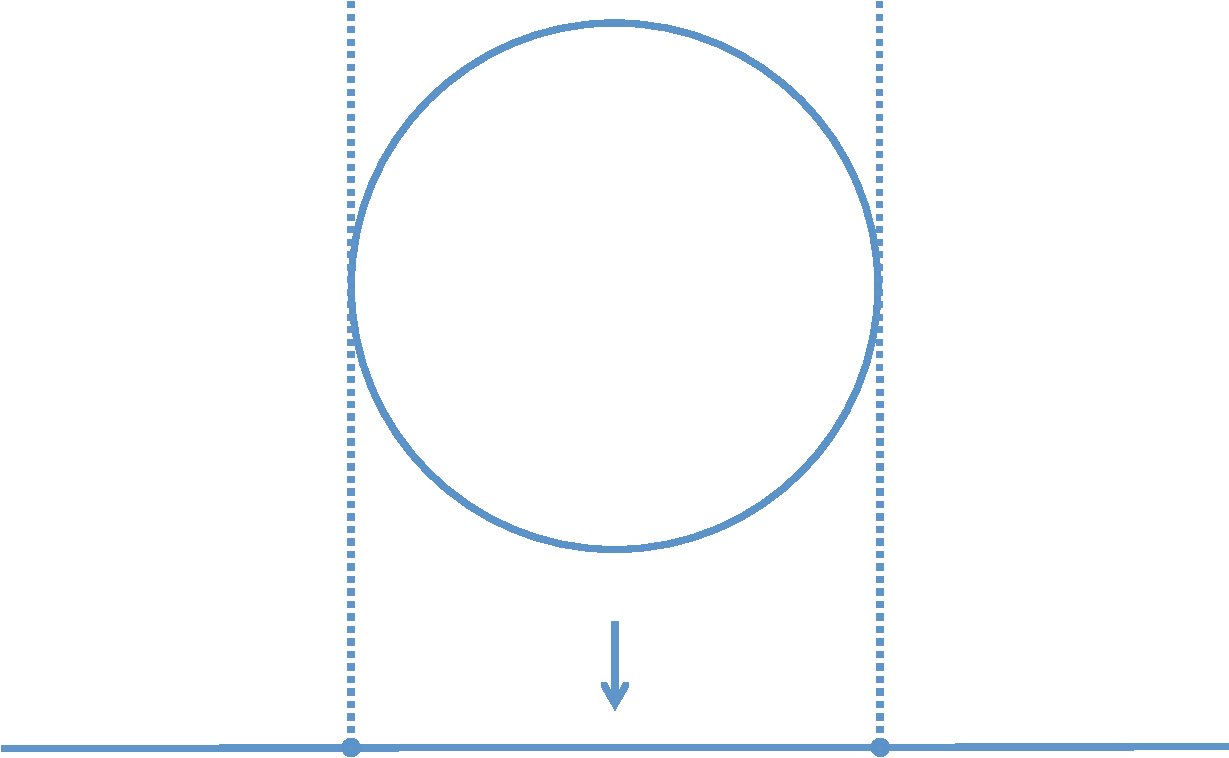
\includegraphics[width=.9\textwidth]{presheaf_1.pdf}
\caption{Height Function on the Circle}
\label{fig:height_circle}
\end{figure}

The definition of level set persistence suffers in one crucial respect. The definition is \emph{non-local} and consequently requires the storage of an infinite amount of data. Consider the map $f$ depicted in Figure \ref{fig:height_circle}. Level set persistence for $H_1$ will assign the zero vector space to every interval of diameter less than $y-x$. Only after inspecting intervals large enough will the topological feature of the circle appear.

A sheaf-theoretic approach to level-set persistence offers the advantage of being local. However, the analogous sheaf version of the level set $H_1$ just examined is the zero sheaf. The trade-off appears to be too great. However, the apparent disadvantage is remedied via the use of sheaf-cohomology, which preserves all the information of the domain space while simultaneously being local.

\section{Approaching Persistence with Sheaves and Cosheaves}

\subsection{Cellular Maps and Absolute Homology Cosheaves}\label{subsec:abs_homology_cosheaves}

The contravariant nature of sheaves should remind us that that they are most naturally associated with cohomology of a space. Cosheaves, being covariant with respect to the inclusion of opens, are naturally associated with homology of a space. Since we are working over a field, we can pass back and forth between these perspectives. However, to coincide with the traditional use of homology in persistence, we first introduce our version of persistence using cosheaves.

\begin{defn}\label{defn:abs-hom-cosheaf}\index{absolute homology cosheaf}\index{cosheaf!absolute homology}
Suppose $X$ and $Y$ are cell complexes and $f:Y\to X$ is a \emph{proper} cellular map, see Definition \ref{defn:cell_map} for a reminder, then for each natural number $i\geq 0$ we have the following $i$th \textbf{absolute homology cosheaf} $\hF_i$, which assigns to a cell $\sigma$ in $X$ the $i$th homology of the pre-image $f^{-1}(\st(\sigma))$, i.e.
\[
	\hF_i(\sigma):=H_i(f^{-1}(\st(\sigma));k).
\]
This is clearly a cellular cosheaf since if $\sigma\leq \tau$, then $\st(\tau)\subseteq \st(\sigma)$ and thus we have a map 
\[
r_{\sigma,\tau}:H_i(f^{-1}(\st(\tau));k) \to H_i(f^{-1}(\st(\sigma));k).
\]
\end{defn}

\begin{figure}
\begin{center}
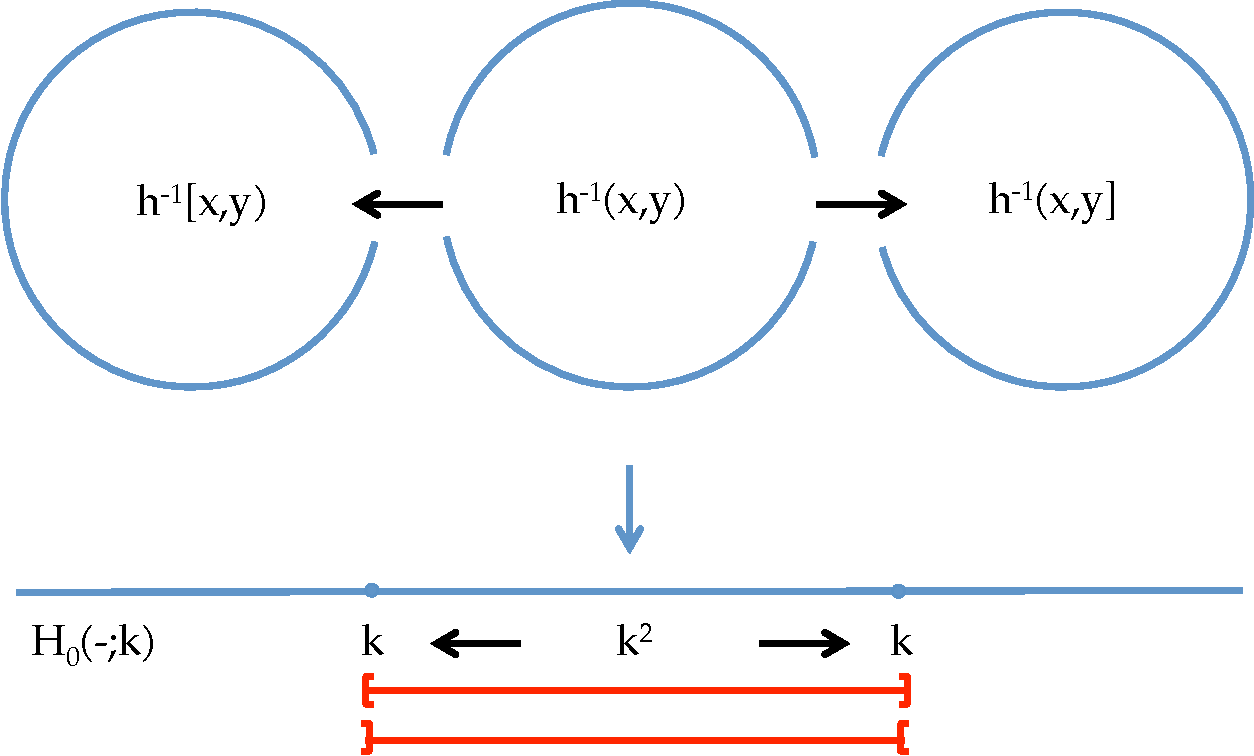
\includegraphics[width=\textwidth]{levelset_open_ex20pt.pdf}
\end{center}
\caption{Homology Cosheaf for a circle, with barcodes}
\label{fig:circle_bc}
\end{figure}

By Corollary \ref{cor:sheaves_remak} we know that every absolute homology cosheaf can be decomposed into indecomposable sheaves. For cellular maps $f:Y\to X$ where $X$ is a compact subset of $\R$, the absolute homology cosheaves have the following form:
\[
H_i(f^{-1}(\st(x_0));k) \leftarrow H_i(f^{-1}((x_0,x_1));k) \rightarrow H_i(f^{-1}(\st(x_1));k) \leftarrow \cdots
\]
Hence, by Gabriel's Theorem \ref{thm:gabriel} absolute homology cosheaves over $X\subset \R$ can be assigned barcodes. However, by inspecting the support of these indecomposable cosheaves we observe that there are four types of bars that make up any barcode:
\[
	[\textrm{---}] \qquad (\textrm{---}) \qquad [\textrm{---}) \qquad (\textrm{---}]
\]

\begin{ex}
Let $h:S^1\to\R$ be the standard height function on the circle, drawn in Figure \ref{fig:height_circle}. The only absolute homology cosheaf of interest is $\hF_0$, since the fibers have no higher homology. The associated pre-images, values of the homology cosheaf and barcode are drawn in Figure \ref{fig:circle_bc}.
\end{ex}

\begin{rmk}[Barcode Notation]
We will use intervals to represent barcodes and these will be sensitive to whether the first or last vector space in an indecomposable representation falls on a vertex or an open interval in some stratification of $[0,1]$ or $\RR$. For visual clarity, we will adopt the convention that a turned around square bracket is equivalent to a round one, i.e. $(x_i,x_{i+1})\rightsquigarrow ]x_{i},x_{i+1}[$ and $[x_i,x_{i+1})\rightsquigarrow [x_i,x_{i+1}[$ and so on.
\end{rmk}

By viewing these barcodes as cosheaves, which have a homology theory, we can compute barcode homology.

\begin{lem}\label{clm:BM_barcodes}\index{homology!of a cellular cosheaf!via barcodes}\index{cosheaf!cellular!homology via barcodes}
	Suppose $X$ is a compact subset of $\R$, equipped with some cell structure. The cosheaf homology of the four types of indecomposable cosheaves coincides with the Borel-Moore homology of the underlying barcode, i.e.
	\[
		H_0^{BM}([\textrm{---}])=k \qquad H_1^{BM}(]\textrm{---}[)=k \qquad H_i^{BM}([\textrm{---}[)=H_i^{BM}(]\textrm{---}])=0
	\]
	with all other Borel-Moore homology groups being zero. Moreover, since cosheaf homology commutes with finite direct sums, cellular cosheaf homology of $\hF$ on $X$ can be computed using the barcode $B_{\hF}$ associated to the Remak decomposition of $\hF$.
	\[
		H_i(X;\hF)\cong \oplus H_i^{BM}(B_{\hF}) \qquad i=0,1
	\]
	In short,
	\begin{quote}
	\centering
	{\em $H_0(X;\hF)$ counts \textbf{closed bars} and $H_1(X;\hF)$ counts \textbf{open bars}.}
	\end{quote}
	
\end{lem}
\begin{proof}
The proof of the claim uses simple computations, illustrated in the examples, and an invariance under subdivision argument, which is proved in Theorem \ref{thm:subdivision}. The true sticking point is why ordinary cosheaf homology becomes Borel-Moore (cosheaf) homology, which is developed in section \ref{subsubsec:BM_cosheaf_homology}.

If we imagine that we are extending the constant cosheaf supported on a barcode to a cosheaf defined on all of $[0,1]$, then the natural way of extending by zero is to use the pushforward with open supports functor $j_{\dd}$, where
\[
	j: B \hookrightarrow [0,1] \qquad \mathrm{and} \qquad \hat{k}_B \mapsto j_{\dd}\hat{k}_B.
\]
The process of taking cosheaf homology is to then push forward this cosheaf to a point. However, using Lemma \ref{lem:BM_cosheaf_homology} we see the following is true: 
\[
	p_!\hat{k}_B \cong p_* j_{\dd}\hat{k}_B \qquad H^{BM}_i(B;\hat{k}_B)\cong H_i([0,1];j_{\dd}\hat{k}_B)
\]
When it is clear that we are working on $[0,1]$ we may write $\hat{k}_B$ instead of $j_{\dd}\hat{k}_B$.
\end{proof}

One of the advantages of absolute homology cosheaves is that over the real line they can be used to compute the homology of the domain.

\begin{cor}[``The Barcode Trick'']\label{cor:barcode_homology}\index{barcode!trick}
	Assume $Y$ is compact and $f:Y\to X$ is a cellular map with $f(Y)=X\subset\RR$. For each $i$, let $B_i$ denote the barcode associated to the $i$th absolute homology cosheaf. The following is true:
	 \[
	  H_i(Y;k)\cong H_0(X;\hF_i)\oplus H_1(X;\hF_{i-1}) \cong H_0^{BM}(B_i)\oplus H_1^{BM}(B_{i-1})
	 \]
\end{cor}
\begin{proof}
This is an immediate corollary of Theorem \ref{thm:leraysheaf} and Lemma \ref{clm:BM_barcodes}.
\end{proof}

\begin{ex}[Height function on the Two Sphere]

\begin{figure}
\begin{center}
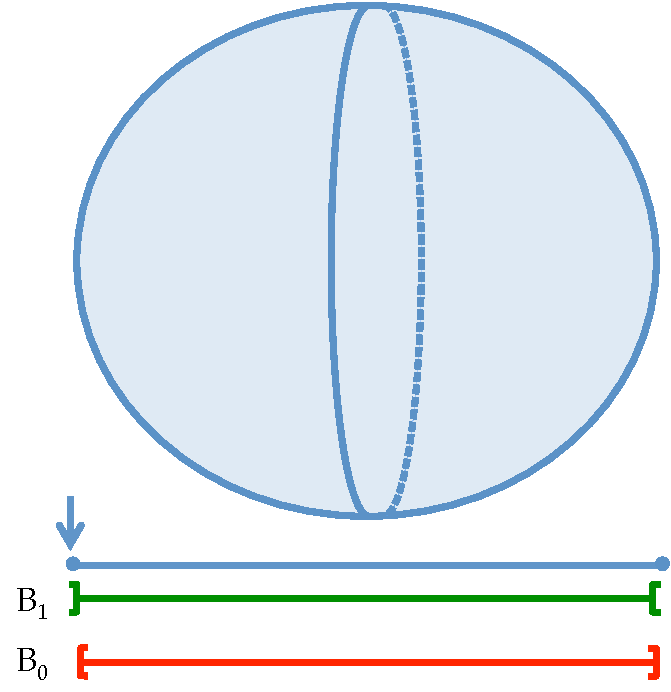
\includegraphics[width=.7\textwidth]{sphere_bc.pdf}
\end{center}
\caption{Barcodes and the Two Sphere}
\label{fig:sphere_bc}
\end{figure}

Let $h:S^2\to\RR$ be the standard height function on the two sphere. In Figure \ref{fig:sphere_bc} we have drawn the map and the associated barcodes. The barcode decomposition for the cosheaf associated to taking $H_0$ of the fiber is trivial because it is already an indecomposable cosheaf.
\[
	\hF_0: \qquad \xymatrix{k & \ar[l] k \ar[r] & k}
\]
Similarly, taking $H_1$ of the fiber also yields an indecomposable cosheaf
\[
	\hF_1: \qquad \xymatrix{0 & \ar[l] k \ar[r] & 0}
\]

Now let us compute cosheaf homology. Since the space $X=[0,1]$ is compact, ordinary and compactly supported cosheaf homology agree. We label our cells as $x=0$, $a=(0,1)$ and $y=1$. To get an ordered basis and matrix representatives for our homology computation, we choose the local orientation pointing to the right and use the lexicographic ordering on the cells. For $\hF_0$ we get the following boundary matrix and homology groups:
\[
  \partial_1=\begin{bmatrix}-1 \\ 1\end{bmatrix} : k_a \to k_x\oplus k_y \qquad \Rightarrow \qquad H_1(X;\hF_0)=0 \quad H_0(X;\hF_0)=k.
\]
For $\hF_1$ the computation is even easier:
\[
  \partial_1: k_a \to 0 \qquad \Rightarrow \qquad H_1(X;\hF_1)=k \quad H_0(X;\hF_1)=0
\]
One can then check \ref{cor:barcode_homology} simply as follows:
\[
\xymatrix{H_0(X;\hF_1)=0 \ar@{.}[rd] & H_1(X;\hF_1)=k \\
H_0(X;\hF_0)=k & H_1(X;\hF_0)=0}
\]

\[
H_0(S^2)=k \qquad H_1(S^2)=0 \qquad H_2(S^2)=k
\]
\end{ex}

\begin{ex}[Height function on a Cone]

\begin{figure}[ht]
\centering
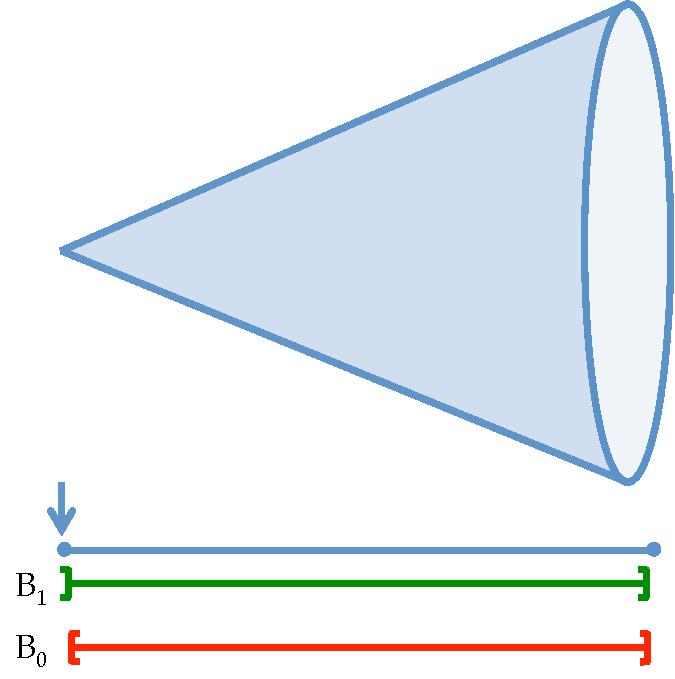
\includegraphics[width=.7\textwidth]{cone_bcp.pdf}
\caption{Barcodes for the Cone}
\label{fig:cone_bc}
\end{figure}

The height function on a cone is not a Morse function because differentiability breaks down at the cone point; see Figure \ref{fig:cone_bc}. One could use stratified Morse theory as a substitute, but we'll use cosheaf homology. Here the cosheaf $\hF_0$ is the same as the previous example; we will not repeat the computation. The cosheaf $\hF_1$
\[
	\hF_1: \qquad \xymatrix{0 & \ar[l] k \ar[r] & k}
\]
exhibits different behavior. The cosheaf homology computation for this cosheaf reveals that the half-open barcode, embedded inside a compact interval, has no non-zero homology groups.
\[
  \partial_1=\id: k_a \to k_y \qquad \Rightarrow \qquad H_1(X;\hF_1)=0 \quad H_0(X;\hF_1)=0
\]
Checking \ref{cor:barcode_homology} again gives
\[
\xymatrix{H_0(X;\hF_1)=0 \ar@{.}[rd] & H_1(X;\hF_1)=0 \\
H_0(X;\hF_0)=k & H_1(X;\hF_0)=0}
\]

\[
H_0(C)=k \qquad H_1(C)=0 \qquad H_2(C)=0
\]
\end{ex}



Let's illustrate the utility of the barcode trick by computing cosheaf homology over $X$ using two different methods:
\begin{itemize}
	\item Using the computational formulae of section \ref{subsec:comp_homology}
	\item Determining the barcode decomposition and applying claim \ref{clm:BM_barcodes}.
\end{itemize}

\begin{ex}[Height function on the Torus]

\begin{figure}[ht]
\centering
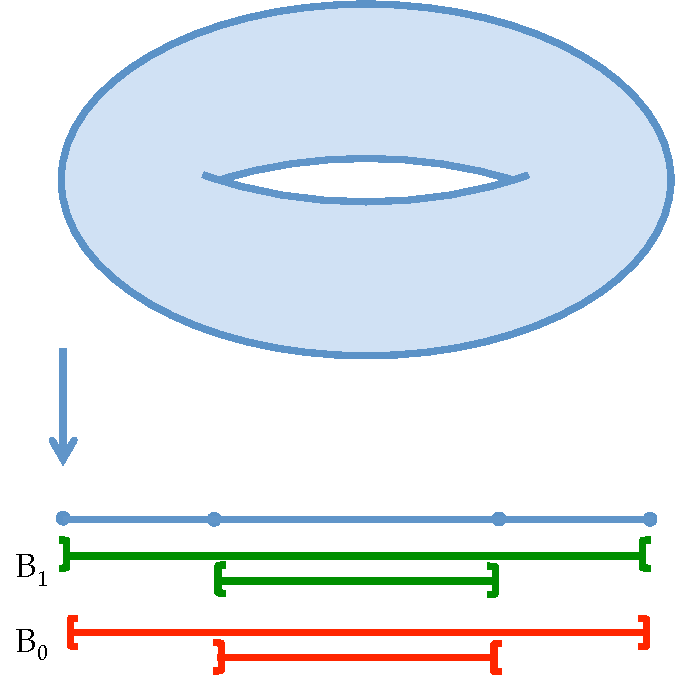
\includegraphics[width=.7\textwidth]{torus_bc.pdf}
\caption{Barcodes for Bott's torus}
\label{fig:torus_bc}
\end{figure}

The standard introductory example of Morse theory, first popularized by Raoul Bott, is the height function on the torus. In Figure \ref{fig:torus_bc} we have drawn the behavior of the fibers over the critical values and the non-critical intervals. For the sake of brevity, let us write out only the cosheaf $\hF_1$:
\[
\xymatrix{0 & \ar[l] k_a \ar[r] & k_y^2 & \ar[l] k_b^2 \ar[r] & k_z^2 & \ar[l] k_c \ar[r] & 0}
\]
Here the maps from $k_a$ to $k_y^2$ and $k_c$ to $k_z^2$ are the diagonal maps
\[
 r_{z,a}=\begin{bmatrix}1 \\ 1\end{bmatrix}=r_{z,c}
\]
and the other maps are the identity. Choosing the orientation that points to the right, we get the follow matrix representation for the boundary map:
\[
	\partial_1=\begin{bmatrix}1 & -1 & 0 & 0 \\
					1 & 0 & 1 & 0 \\
					0 & 1 & 0 & -1 \\
					0 & 0 & 1 & -1
	\end{bmatrix}
	\qquad H_1(X;\hF_1)=<\begin{bmatrix} 1 \\ 1 \\1 \\1\end{bmatrix}> \qquad H_0(X;\hF_1)\cong k
\]
However, if we change our bases as follows
\[
	\begin{bmatrix} y_1'= y_1 \\ y'_2=y_1+y_2\end{bmatrix} \qquad \begin{bmatrix} b_1'= b_1 \\ b'_2=b_1+b_2\end{bmatrix} \qquad \begin{bmatrix} z_1'= z_1 \\ z'_2=z_1+z_2\end{bmatrix}
\]
then our cosheaf $\hF_1$ can then be written as the direct sum of two indecomposable cosheaves:
\[
\xymatrix{0 & \ar[l] 0 \ar[r] & k_{y'_1} & \ar[l] k_{b'_1} \ar[r] & k_{z'_1} & \ar[l] 0 \ar[r] & 0}
\]
\[
\xymatrix{0 & \ar[l] k_a \ar[r] & k_{y'_2} & \ar[l] k_{b'_2} \ar[r] & k_{z'_2} & \ar[l] k_c \ar[r] & 0}
\]
Hence it is apparent that
\[
	H_i(X;\hF_1)\cong H_i^{BM}([\textrm{---}])\oplus H_i^{BM}(]\textrm{---}[).
\]
From which the homology of the torus can be directly observed.
\[
\xymatrix{H_0(X;\hF_1)=k \ar@{.}[rd] & H_1(X;\hF_1)=k \\
H_0(X;\hF_0)=k & H_1(X;\hF_0)=k}
\]
\[
H_0(T)=k \,\, H_1(T)=k^2 \,\, H_2(T)=k
\]
\end{ex}

\subsection{Local-to-Global Computations via Cellular Sheaves}
\label{subsec:local-to-global}

Aside from the decoration of cosheaves, section \ref{subsec:abs_homology_cosheaves} is completely classical and can be stated much more generally using non-cellular sheaves and cosheaves. However, one can still use cellular versions to compute homological information of non-cellular spaces as already noted by the author in~\cite{DMT_sheaves}.\index{discrete Morse theory for sheaves}

\subsubsection{The \v{C}ech Approach}

Recall that any topological space $X$ equipped with a cover $\cU$ has an associated simplicial approximation $N_{\cU}$ given by the nerve construction considered in Definition \ref{defn:nerve}. The nerve theorem tells us when this approximation is ``good enough'' for the purposes of cohomology.

\begin{thm}[Nerve Theorem \cite{leray45,borsuk-nerve}]\index{nerve theorem}
Given a topological space $X$ and a cover $\cU$, if the support $U_\sigma \subset X$ of each $\sigma \in N_\cU$ is acyclic (i.e., the reduced cohomology $\tilde{H}^\bullet(U_\sigma;R) = 0$ vanishes),
then $H^\bullet(N_\cU;R)\cong H^\bullet(X;R)$.
\end{thm}

Typically, the coarsest covers do not satisfy the acyclicity assumption. One achieves this by refinement of the cover, with the additional cost of more simplices in $N_{\cU}$. However, one can dodge this refinement by recording the cohomology of the intersection as a cellular sheaf on $N_{\cU}$.

\begin{defn}[\v{C}ech Sheaves]\index{sheaf!C@\v{C}ech}\index{Cech@\v{C}ech sheaves}

The {\bf \v{C}ech cellular sheaves} $\Cech^n$ associated to the cover $\cU$ of a space $X$ are defined on the nerve $N_\cU$ by the following data. Each $\sigma \in N_\cU$ is assigned the vector space $\Cech^n(\sigma) = H^n(U_{\sigma};k)$ and each face relation $\sigma \subset \tau$ is assigned the linear map $\Cech^n_{\sigma\tau}: H^n(U_{\sigma};R)\to H^n(U_{\tau};R)$ arising from the inclusion of supports $U_\tau \hookrightarrow U_\sigma$.

\end{defn}

If all simplex supports are acyclic, then $\Cech^0$ reduces to the constant sheaf on $N_{\cU}$ and all other $\Cech^n$s are trivial; in the absence of acyclicity assumptions, the following result yields a simple correction.

\begin{prop}
\label{prop:cechsheaf}
Let $X$ be a topological space and $\cU$ a cover whose nerve $N_\cU$ is at most one-dimensional. Then, for each $n \in \N$,
\begin{equation*}
		H^n(X;k) \cong H^0(N_\cU;\Cech^n)\oplus H^1(N_\cU;\Cech^{n-1}).
\end{equation*}
\end{prop}

We note that similar results have been obtained by Burghelea and Dey~\cite{dey_circle}, as well as Carlsson, de Silva, and Morozov~\cite{pyramid} in the context of zig-zag persistence. The difference between their results and ours is that their results depend on the decomposition of zig-zag persistence modules into indecomposable modules (barcodes). Our result makes the recognition that these modules are rightly conceived as sheaves over a linear nerve with a cohomology that can be quickly computed using discrete Morse theory~\cite{DMT_sheaves}.

Proposition \ref{prop:cechsheaf} generalizes the familiar Mayer-Vietoris long exact sequence, as the next example shows.
\begin{ex}[Mayer-Vietoris]\index{Mayer-Vietoris!via cellular sheaf cohomology}
The Mayer-Vietoris Theorem states that given an open cover of $X$ by two open sets $\cU=\{A,B\}$ we have the following exact sequence of $R$-modules and maps:

\[
\xymatrix{
	            0\ar@{->}[r] & H^0(X)\ar@{->}[r] & H^0(A)\oplus H^0(B) \ar@{->}[r]
	                   & H^0(A\cap B) \ar `r[d] `_l[lll] ^{\psi^0} `^d[dlll] `^r[dll] [dll] \\
	            & H^1(X)\ar@{->}[r] & \hspace{12pt}\cdots\hspace{12pt}\ar@{->}[r]
	                   & H^{n-1}(A\cap B) \ar `r[d] `_l[lll] ^{\psi^{n-1}} `^d[dlll] `^r[dll] [dll] \\
	            &H^{n}(X)\ar@{->}[r] & H^{n}(A)\oplus H^{n}(B) \ar@{->}[r]
	                   & H^{n}(A\cap B) \ar `r[d] `_l[lll] ^{\psi^{n}} `^d[dlll] `^r[dll] [dll] \\
	            & & \cdots &
	}
\]
Ideally one can determine the unknown cohomology of $X=A\cup B$ by inspecting the terms on either side. More formally, one uses universal constructions to force $H^n(X)$ into a more manageable short exact sequence:
\[
	\xymatrix{ & H^{n-1}(A)\oplus H^{n-1}(B) \ar[r]^-{\delta^0_{n-1}} & H^{n-1}(A\cap B) \ar[d] \ar[ld] & 0 \ar[d] &  \\
	0 \ar[r] & \cok(\delta^0_{n-1}) \ar[d] \ar@{.>}[r] & H^n(X) \ar@{.>}[r] \ar[d] & \ker(\delta^0_n) \ar[r] \ar[ld] & 0 \\
	& 0 & H^n(A)\oplus H^n(B) \ar[r]^-{\delta^0_{n}} & H^n(A\cap B) &  }
\]
The dotted maps are defined by the universal property of the cokernel and kernel, respectively. Over an arbitrary coefficient ring $R$ we would have to solve an extension problem in order to infer $H^n(X)$. If we take $R$ to be a field $k$, then every short exact sequence splits and we can deduce that
\[
	H^n(X)\cong \ker(\delta^0_n)\oplus \cok(\delta^0_{n-1})\cong H^0(N_{A,B};\Cech^n)\oplus H^1(N_{A,B};\Cech^{n-1})
\]
where $N_{A,B}$ is the unit interval, viewed as the nerve of a two-element cover.
\end{ex}

\subsubsection{The Leray Approach}

As Section~\ref{subsec:abs_homology_cosheaves} already indicated with examples, one can compute homological information of a space $Y$ with a suitably nice map $f:Y\to X$. We view this construction from a different perspective. By assuming that $X$ comes with a cover $\cV$, having nerve $N_\cV$, one can pull-back the associated \v{C}ech sheaf on $N_\cV$ along $f$ to yield local information about $Y$.

\begin{defn}[Leray Sheaves]\index{sheaf!Leray}\index{Leray sheaves}
The {\bf Leray cellular sheaves} $\Leray^n$ associated to a map $f:Y\to X$ and a cover $\cV$ of $f(Y) \subset X$ are defined over the nerve $N_\cV$ as follows. Each simplex $\sigma \in N_\cV$ is assigned the cohomology of the preimage of its support, i.e., $\Leray^n(\sigma) = H^n(f^{-1}(V_\sigma);k)$; furthermore, each face relation $\sigma \subset \tau$ is assigned the map induced on cohomology by the inclusion $f^{-1}(V_\tau) \hookrightarrow f^{-1}(V_\sigma)$.
\end{defn}
\begin{rmk}
\begin{itemize}
\item We will sometimes use the notation $F^n$ in place of $\Leray^n$ to emphasize the association to $f:Y\to X$. 
\item The absolute homology cosheaf $\hF^n$ of Definition \ref{defn:abs-hom-cosheaf} is clearly the cosheaf-theoretic version of $\Leray^n$ when the cover is given by the open stars of the cells.
\item A More general version of the Leray sheaf is given by the right derived pushforward of the constant sheaf along the map $f$.
\end{itemize}
\end{rmk}

In the special case where $X = Y$ and $f$ is the identity map, the Leray sheaves clearly coincide with the \v{C}ech sheaves associated to the cover $\cV$ of $X$. Thus, the following result generalizes Proposition \ref{prop:cechsheaf}.

\begin{thm}
\label{thm:leraysheaf}
	Let $f:Y \to X$ be continuous. Assume a cover $\cV$ of the image $f(Y) \subset X$ whose nerve $N_\cV$ is at most one-dimensional. Then, for each $n \in \N$,
\begin{equation*}
		H^{n}(Y;k) \cong H^0(N_\cV;\Leray^n) \oplus H^1(N_\cV;\Leray^{n-1}) .
\end{equation*}
\end{thm}
\begin{proof}
		The theorem is a simple consequence of the Leray spectral sequence which packages the cohomology of $Y$ into a coefficient system over the space $X$ from a map $f:Y\to X$~\cite{mccleary}. The restriction to a one-dimensional nerve forces the spectral sequence to collapse on the second page and hence yield the desired isomorphisms. More precisely, for each open $V\subset f(Y)$, let $C^n(V;R)$ denote the vector space freely generated by the set of all cochains defined on $V$. Clearly if $V \subset U$, then there is a surjection $C^n(U;R) \to C^n(V;R)$ defined by restriction of cochains. The sheaf $\widetilde{C}^n$ associated to this presheaf of singular cochains is consequently {\em flabby} (see \cite[p.~97]{ramanan2005global}).
		
Consider the following double complex of vector spaces:
	\[
	 \xymatrix{ \vdots & \vdots & \vdots & \vdots\\
	C^2(Y) \ar[r] \ar[u] & \bigoplus_{\dim \sigma = 0} \widetilde{C}^2(f^{-1}(V_\sigma)) \ar[r] \ar[u] & \bigoplus_{{\dim \tau = 1}} \widetilde{C}^2(f^{-1}(V_\tau) \ar[r] \ar[u] & 0 \\
	C^1(Y) \ar[r] \ar[u] &\bigoplus_{\dim \sigma = 0} \widetilde{C}^1(f^{-1}(V_\sigma)) \ar[r] \ar[u] & \bigoplus_{\dim \tau = 1} \widetilde{C}^1(f^{-1}(V_\tau) \ar[r] \ar[u]  & 0 \\
	C^0(Y) \ar[r] \ar[u] & \bigoplus_{\dim \sigma = 0} \widetilde{C}^0(f^{-1}(V_\sigma)) \ar[r] \ar[u] & \bigoplus_{\dim \tau = 1} \widetilde{C}^0(f^{-1}(V_\tau)) \ar[r] \ar[u] & 0 }
	\]
	It follows from standard results \cite[Thm~II.5.5, Thm~III.4.13]{Bredon}) that the rows are exact. By the acyclic assembly lemma \cite{weibel}, the spectral sequence converges to the cohomology of the leftmost column, i.e., $H^\bullet(Y;k)$. If one takes cohomology in the vertical direction, one obtains the defined cochain groups associated to the Leray cellular sheaves $\Leray^n$:
	\[
	 \xymatrix{  \vdots & \vdots & \vdots\\
	\bigoplus_{\dim \sigma = 0} H^2(f^{-1}(V_\sigma)) \ar[r] & \bigoplus_{\dim \tau = 1} H^2(f^{-1}(V_\tau)) \ar[r] & 0 \\
	\bigoplus_{\dim \sigma = 0} H^1(f^{-1}(V_\sigma)) \ar[r] & \bigoplus_{\dim \tau = 1} H^1(f^{-1}(V_\tau)) \ar[r]  & 0 \\
	\bigoplus_{\dim \sigma = 0} H^0(f^{-1}(V_\sigma)) \ar[r] & \bigoplus_{\dim \tau = 1} H^0(f^{-1}(V_\tau)) \ar[r] & 0}
	\]
Taking cohomology horizontally corresponds precisely to computing separately (in parallel, if one wishes) the cohomology of the Leray sheaves $\Leray^n$ over $N_\cV$, thus producing the final stable page of the spectral sequence.
	\[
	 \xymatrix{  \vdots & \vdots & \vdots\\
	 H^0(N_\cV; \Leray^2) & H^1(N_\cV;\Leray^2) & 0 \\
	 H^0(N_\cV; \Leray^1) \ar[rru] & H^1(N_\cV;\Leray^1)  & 0 \\
	 H^0(N_\cV; \Leray^0) \ar[rru] & H^1(N_\cV;\Leray^0) & 0}
	\]
Over a general ring $R$, these terms prescribe a filtration of the cohomology, giving rise to extension problems; however, over a field $k$ one can read off the cohomology directly.
\end{proof}

Note that the proof indicates precisely where we require the one-dimensional nerve restriction. Without this assumption in place, the second page of the spectral sequence may not be stable and the conclusion of the theorem need not hold.

\subsubsection{A Unifying Perspective}

There is a more sophisticated version of the nerve described originally by Segal~\cite{segal_CSSS} which is homotopically faithful to the underlying space independent of the particulars of the cover. This notion has been used in recent applications~\cite{zomorodian2008localized} and parallelizations for homology computation~\cite{lewis2012multicore}.

\begin{defn}[Mayer Vietoris Blowup]\label{defn:MV_blowup}\index{Mayer-Vietoris!blowup complex}\index{nerve!generalization}
Let $X$ be a topological space equipped with a cover $\cU$ with nerve $N_\cU$. The {\bf Mayer Vietoris blowup} $M_\cU$ associated to $\cU$ is a subset of the product $X \times N_\cU$ defined as follows. The pair $(x,s)$ lies in $M_\cU$ if and only if there is some simplex $\sigma \in N_\cU$ for which $x \in U_\sigma$ and $s \in \sigma$.
\end{defn}

\begin{rmk}
The original description given by Segal is that (up to barycentric subdivision) $M_{\cU}$ is the classifying space of a topological category, whose objects are pairs $(x,U_{\sigma})$ with $x\in U_{\sigma}$ and whose morphisms are pointed inclusions $(x,U_{\sigma})\to (y,U_{\tau})$ where $\tau\subset\sigma\subset I$ and $I$ is the indexing set of the cover $\cU=\{U_i\}_{i\in I}$.
\end{rmk}

Segal provides an updated version of the nerve theorem using this construction~\cite[Prop. 4.1]{segal_CSSS}

\begin{lem}[Generalized Nerve Theorem]\label{lem:generalized_nerve_thm}\index{nerve theorem!generalization}
	If $X$ is a paracompact Hausdorff space and $\cU=\{U_i\}_{i\in I}$ is an open cover of $X$, then $M_{\cU}$ is homotopic to $X$.
\end{lem}
\begin{proof}
An explicit proof is provided by Segal using linear homotopies. Here we take a slightly higher-brow approach.

Being a subset of the product, $M_\cU$ is equipped with natural surjective projection maps
\[
\xymatrix{ ~ & M_\cU \ar[ld]_{\rho_1} \ar[rd]^{\rho_2} & ~\\
X & ~ & N_\cU}
\]
The map $\rho_1$ has contractible fibers: for any $x \in X$, we have $\rho_1^{-1}(x) = \setof{x} \times \sigma_x$ where $\sigma_x$ is the unique simplex of maximal dimension whose support contains $x$. Thus, by Quillen's Theorem A~\cite{quillen1973higher}, the Mayer-Vietoris blowup is homotopy-equivalent to $X$ via $\rho_1$ in full generality.
\end{proof}

On the other hand, it is easy to see that the map $\rho_2$ fails to have contractible fibers precisely when the simplex supports are not contractible. In fact, given $s \in N_\cU$, the fiber $\rho_2^{-1}(s)$ has the homotopy type of the support of $\sigma_s$, which is the unique simplex of maximal dimension whose realization contains $s$. Since cohomology is a homotopy invariant, this leads to the following observation which unifies the \v{C}ech and Leray approaches.

\begin{prop}
The Leray cellular sheaves $\Leray^n$ associated to the map $\rho_2: M_\cU \to N_\cU$, where $N_\cU$ is covered by (small neighborhoods of the topological) simplices $\setof{\sigma}_{\sigma \in N_\cU}$, are isomorphic to the \v{C}ech cellular sheaves $\Cech^n$ associated to the cover $\cU$.
\end{prop}

\begin{rem}
\begin{itemize}
\item The commonality between the \v{C}ech and Leray approaches comes as no surprise to anyone sufficiently familiar with spectral sequences (and would have surprised neither \v{C}ech nor Leray).
\item Both strategies are examples of {\em distributed} cohomology computation because in order to determine the sheaf $\Cech^n$ or $\Leray^n$, one only needs to compute cohomology locally: of a non-trivial intersection of covering sets in the former case, or of a small neighborhood of the fiber $f^{-1}(x)$ in the  latter case. In principle, one can assign each local computation to a different processor, compute the appropriate sheaf cohomology over a decidedly nicer space (either $N_\cU$ or $Y$ depending on the circumstances), and aggregate this information to compute the desired cohomology of $X$.
\item By taking the appropriate linear duals and working with cosheaves, all of our results transform to computations of homology rather than cohomology.
\end{itemize}
\end{rem}

\subsection{Level Set Persistence Determines Sub-level set Persistence}
\label{subsec:level2sub}

\begin{figure}
\begin{center}
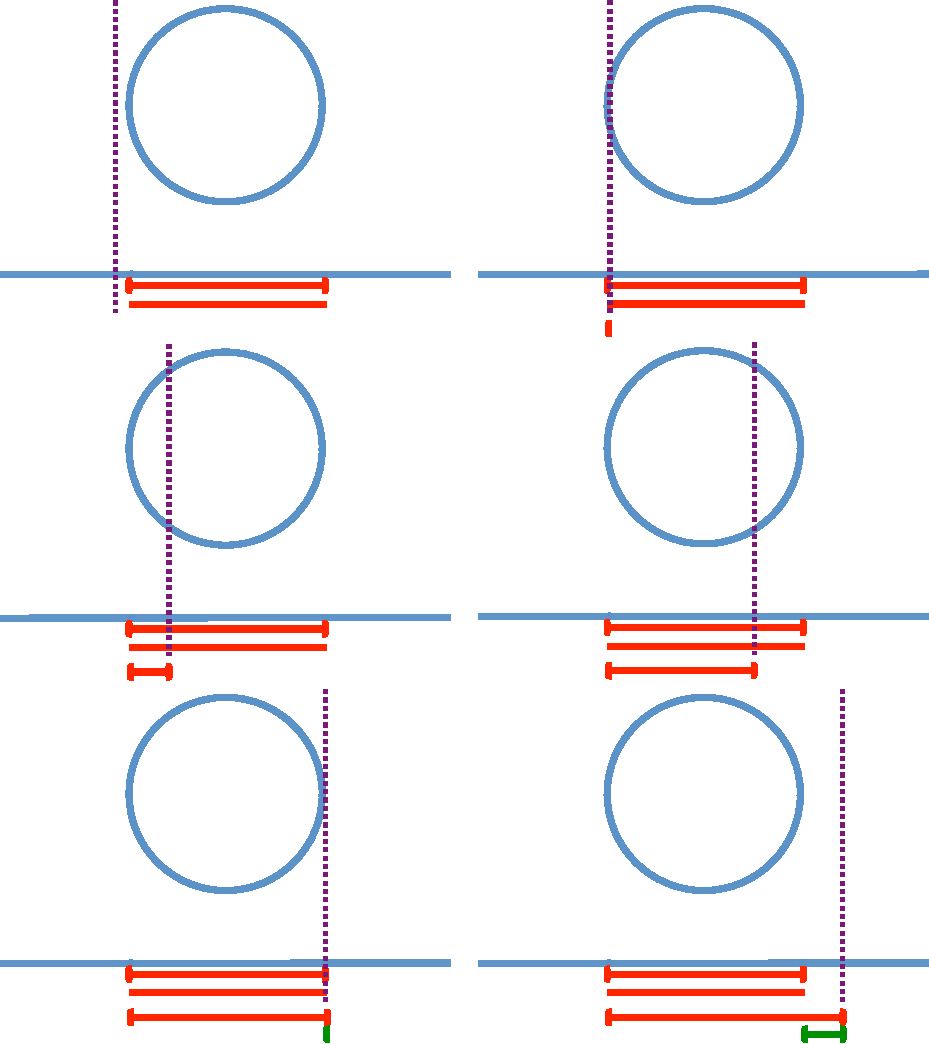
\includegraphics[width=\textwidth]{level_to_sub.pdf}
\end{center}
\caption{Determining Sub-level Set from Level Set Persistence}
\label{fig:level_to_sub}
\end{figure}

We will use Theorem \ref{thm:leraysheaf} to obtain a non-obvious theorem in persistence, namely that level set persistence determines sub-level set persistence. By making use of \ref{clm:BM_barcodes} we illustrate how one can take the absolute homology cosheaves (or Leray sheaves) equipped with a barcode decomposition and sweep from left to right, applying \ref{cor:barcode_homology} to determine the barcodes of the associated sublevel set persistence modules. An example is drawn in Figure \ref{fig:level_to_sub}. Stated formally, we have the following theorem.

\begin{thm}[Level Set to Sublevel Set Persistence]\label{thm:level-to-sub}\index{persistent homology!level set determines sublevel set}
Let $F^k$ denote the Leray sheaf associated to a proper map $f:X\to\R$, whose stalk at $x$ is the cohomology of the fiber $H^k(f^{-1}(x))$. We can define a functor
\[
	S^k:(\RR,\leq)^{op}\to\Vect \qquad S^k(t):=H^0((-\infty,t];F^k)\oplus H^1((-\infty,t];F^{k-1})\cong H^k(f^{-1}(-\infty,t])
\]
whose value records the cohomology of the entire sublevel set. The maps
\[
	S^k(t')\to S^k(t) \qquad t\leq t'
\]
are defined sheaf theoretically by observing that we have maps
\[
	H^0((-\infty,t'];F^k)\to H^0((-\infty,t];F^k) \qquad H^1((-\infty,t'];F^{k-1})\to H^1((-\infty,t];F^{k-1})
\]
the sum of which define the desired map.
\end{thm} 

Observe that since $f:X\to\RR$ is a proper map, the restriction of $f$ to $X_{\leq t}:=f^{-1}((-\infty,t])$ is also a proper map. Consequently, we can apply Theorem \ref{thm:leraysheaf} to the space $X_{\leq t}$ instead, but we have to restrict the sheaves to the subspace $(-\infty,t]$. Fortunately, restriction of a sheaf to a subspace is a standard operation in the Grothendieck six-functor formalism, presented in~\ref{subsec:six_ops}: If $\iota:(-\infty,t]\hookrightarrow \RR$ is the inclusion, then the application of Theorem \ref{thm:leraysheaf} to the restriction reads
\[
	H^k(X_{\leq t};k)\cong H^0((-\infty,t];\iota^*F^k)\oplus H^1((-\infty,t];\iota^*F^{k-1})
\]

The upshot of this formula is that we can define a family of vector spaces, one for each $t\in\RR$ that records the cohomology of the sublevel set $X_{\leq t}$
\[
	S(t):=H^0((-\infty,t];\iota^*F^k)\oplus H_1((-\infty,t];\iota^*F^{k-1})
\]
given by computing sheaf cohomology of the restriction of the Leray sheaves to the subspace $(-\infty,t]$. What remains to be shown is that there are maps
\[
	S(t')\to S(t) \qquad t\leq t'
\]
that can be defined purely sheaf-theoretically. To do this, we will make use of some standard adjunctions in sheaf theory.

\begin{thm}
Let $f:Y\to Z$ be a continuous map. The functors $f^*:\Shv(Z)\to \Shv(Y)$ and $f_*:\Shv(Y)\to\Shv(Z)$ form an adjoint pair $(f^*,f_*)$ and thus
\[
\Hom_{\Shv(Y)}(f^*G,F)\cong \Hom_{\Shv(Z)}(G,f_*F).
\]
\end{thm}

In the above adjunction for sheaves, let $Y=(-\infty,t]$, $Z=(-\infty,t']$ and $f=j$ be the inclusion of $Y$ as a closed subspace of $Z$. Observe that if we set $F=j^*G$ in the above adjunction, then we get an isomorphism
\[
\Hom_{\Shv(Y)}(j^*G,j^*G)\cong \Hom_{\Shv(Z)}(G,j_*j^*G).
\]
that is natural in $G$. This defines the unit of the adjunction:
\[
\id_{\Shv(Y)}\to j_*j^*.
\]
We recall a basic theorem about the pushforward sheaf along a closed immersion~\cite[II.5 p. 102]{iversen}.

\begin{prop}
	For $j:Y\hookrightarrow Z$ the inclusion of a closed subspace, the functor $j_*:\Shv(Y)\to\Shv(Z)$ is exact, i.e. it sends exact sequences of sheaves to exact sequences of sheaves. Moreover, $j^*$ is always exact.
\end{prop}

\begin{lem}
	Suppose $j:Y\hookrightarrow Z$ is the inclusion of a closed subspace and $F$ is a sheaf on $Z$, then there is an induced map from the cohomology of $F$ on $Z$ to the cohomology of $j^*F$ on $Y$.
	\[
		H^i(Z;F)\to H^i(Y;j^*F)
	\]
\end{lem}
\begin{proof}
	We can read off the proof from the following diagram of spaces.
	\[
		\xymatrix{Y \ar@{^{(}->}[rr]^j \ar[dr]_{p_Y} & & Z \ar[ld]^{p_Z} \\ & \ast &}
	\]
	Sheaf cohomology is defined as the right derived functor of pushforward to a point. If we want to compute sheaf cohomology of $F$, one takes an injective resolution of $F$ 
	\[
		0\to F\to I^{\bullet}
	\]
	and applies $p_{Z*}$ to the injective resolution.
	\[
		Rp_{Z*}F:= p_{Z*}I^{\bullet}
	\]
	This results in a chain complex of vector spaces, whose cohomology is the sheaf cohomology of $F$. We usually save this step for last as it takes us out of the category of chain complexes of vector spaces and into the category of graded vector spaces. This is written as follows.
	\[
		R^ip_{Z*}F:=H^i(p_{Z*}I^{\bullet})=:H^i(Z;F)
	\]
	Since $j^*$ is exact we will consider an injective resolution of $F$ and pull that back to an injective resolution of $j^*F$. Observe the following string of identities.
	\begin{eqnarray*}
		Rp_{Y*}j^* F &:=& p_{Y*}j^*I^{\bullet} \\
		&=& (p_{Z}\circ j)_* j^*I^{\bullet} \\
		&=& p_{Z*}j_*j^* I^{\bullet}
	\end{eqnarray*}
	The unit of the adjunction defines a map of sheaves
	\[
		F \to j_*j^*F,
	\]
	which also defines a map on complexes of sheaves and hence injective resolutions.
	\[
		I^{\bullet}\to j_*j^*I^{\bullet}
	\]
	Because $j^*$ and $j_*$ are exact and preserve injectives, $j_*j^*I^{\bullet}$ is an injective resolution of $j_*j^*F$, thus
	\[
		Rp_{Z*}j_* j^* F= p_{Z*}j_*j^* I^{\bullet}= Rp_{Y*}j^* F
	\]
	and hence the unit of the adjunction defines a map
	\[
		Rp_{Z*} F\to Rp_{Y*}j^*F \quad \Rightarrow \quad H^i(Z;F)\to H^i(Y;j^*F.)
	\]
\end{proof}
\begin{rmk}[Abuse of Notation]
	Common practice in the sheaf literature is to suppress the notation $j^*F$ and to just write
	\[
		H^i(Y;F):=H^i(Y;j^*F).
	\]
	The reasoning is that $F$ is a sheaf on $Z$ and hence the only way to parse the formula on the left is to realize that the sheaf must be restricted to the subspace $Y$.
\end{rmk}

As a corollary we obtain our desired result, Theorem \ref{thm:level-to-sub}.

\section{Multidimensional Persistence}

One of the single greatest theoretical challenges to topological data analysis is a foundation for multi-dimensional persistence~\cite{lesnick-thesis}. To consider why data analysts might want such a thing, consider the following example.

Suppose $X$ is the shape depicted in Figure \ref{fig:flare_holes}. A common feature of interest in applications~\cite{lum2013extracting} is the presence of \emph{flares} or \emph{tendrils}. Sublevel set persistence provides a method for detecting such features. Consider the \textbf{$p$th eccentricity functional} on $X$:
\[
E^p(x):=\left(\int_{y\in X} d(x,y)^p dy\right)^p.
\]

If we filter by superlevel sets, the four endpoints of the perceived flares in Figure \ref{fig:flare_holes} will come into view. Said using homology, there are a suitable large range of values $t$ for which $E^p_{\geq t}:=\{x\in X\,|\, E^p(x)\geq t\}$ will have
\[
H_0(E^p_{\geq t};k) \cong k^4.
\]
This formally expresses the four flare-like features we see in the space $X$.

Now suppose that we are not just interested in the number of eccentric features, but rather we are interested in holes with high eccentricity value, i.e. the persistence module
\[
H_1(E^p_{\geq t};k)
\]
is of interest. However, what size of hole is of interest, and what can be regarded as noise? In other words, what is the behavior of the two-parameter family of vector spaces
\[
MP_1(t,r):=H_1((E^p_{\geq t})^r;k)
\]
where $Y^r$ denotes the set of points within distance $r$ of a subspace $Y$. This family of vector spaces defines a functor
\[
MP_1:(\R^2,\leq)\to \Vect \qquad \mathrm{where} \qquad MP_1(t,r):=H_1((E^p_{\geq t})^r;k)
\]
where $\R^2$ is viewed as a poset under the relation $(t,r)\leq (t',r')$ if and only if $t'-t$ and $r'-r$ are non-negative numbers. 

\begin{figure}[ht]
\begin{center}
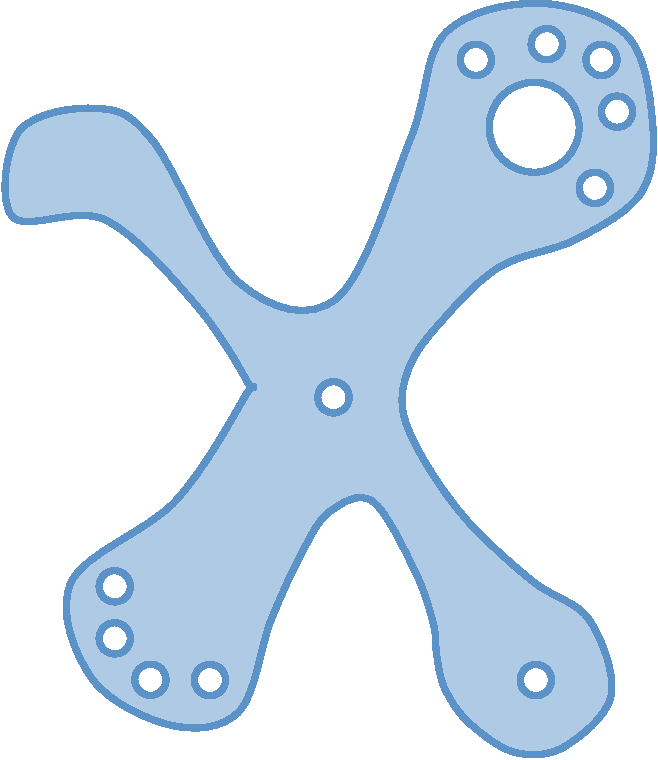
\includegraphics[width=.7\textwidth]{flare_holes.pdf}
\end{center}
\caption{A Shape Described with Multi-D Persistence}
\label{fig:flare_holes}
\end{figure}

This gives the general definition of a multidimensional persistence module as introduced in~\cite{carlsson2009theory}.

\begin{defn}[Multi-dimensional Sub-Level Set Persistence]\index{persistent homology!multi-dimensional!sublevel set}
Suppose we are given a map $f:X\to\R^n$, with coordinate functions $f(x)=(f_1(x),\ldots,f_n(x))$. The \textbf{$i$th multidimensional persistence module} is defined to be the functor
\[
MP_i:(\R^n,\leq) \to \Vect \qquad (t_1,\ldots,t_n)\rightsquigarrow H_i(\{x\in X\,|\,f_j(x)\leq t_j,\, 1\leq j\leq n\};k)
\]
\end{defn}

\subsubsection{Critique of the Definition of Multi-D Persistence}

There are a few problems that such a definition suffers from:
\begin{itemize}
\item Such a definition is strongly dependent on the particular choice of basis given to $\R^n$. If one is given an abstract function $f$, valued in say a manifold $M$, then the definition fails.
\item The definition is not local.
\item There is no decomposition theorem akin to Theorem \ref{thm:crawleyboevey}. There are no barcodes. This is fundamentally due to Gabriel's Theorem \ref{thm:gabriel}, but an explicit example is provided in~\cite[Sec.5.2]{carlsson2009theory}, which suggests other invariants as well.
\end{itemize}

Sheaves and cosheaves overcome the first problem by putting level set persistence as the primary object of interest. Locality is also provided by using sheaves. Our definition of a multi-dimensional persistence module is simply the Leray sheaf.

\begin{defn}[Multi-D Persistence as the Derived Pushforward]\index{persistent homology!multi-dimensional!via derived pushforward}
Suppose $f:Y\to X$ is a continuous map. The right derived pushforward of the constant sheaf $Rf_*k_Y$ is gotten by taking a resolution of $k_Y$ by the complex of singular cochains $\widetilde{C}^{\bullet}$ and pushing forward along $f$. The Leray sheaves are the $n$th cohomology sheaves of this complex, i.e.
\[
F^n:=\cH^n(f_*\widetilde{C}^{\bullet})=:R^nf_*k_Y.
\]
If $f$ is proper, then the stalks of $F^n$ record the cohomology of the level set, i.e. $F^n_x\cong H^n(f^{-1}(x);k)$. We define \textbf{$n$th multi-dimensional level set persistence} of a \emph{proper} map $f:Y\to X$ to be the Leray sheaf $F^n$.
\end{defn}

\begin{rmk}
 If $f$ is not proper, then one can use the pushforward with compact supports to encode the compactly supported cohomology of the fiber.
\end{rmk}

One can always obtain the traditional sub-level set definition from this definition by using a multi-dimensional version of Theorem \ref{thm:level-to-sub}, the Leray spectral sequence.

Sheaves also suffer from the lack of a nice set of indecomposables, but the Grothendieck operations provide one possible approach.

\subsection{Generalized Barcodes}
\label{subsec:barcode_ss}

The need for a generalized notion of a barcode comes from the need to communicate topological summaries to non-topologists. A scientist can easily understand a histogram and the barcode is only subtly different from a histogram.

\begin{defn}[Generalized Barcodes]\label{defn:generalized_bc}\index{barcode!generalized}\index{decomposition!generalized barcode}
	Suppose $F^n$ is the Leray sheaf associated to a proper map $f:Y\to X$. A \textbf{generalized barcode} for $F^n$ is the expression of $F$ as follows.
	\[
	F^n\cong \bigoplus_{b\in B} (j_b)_! k_{Z_b}
	\]
	where $j_b:Z_b\to X$ are maps indexed by the barcode $B$ and where each $(j_b)_! k_{Z_b}$ is assumed to be indecomposable.
\end{defn}
\begin{rmk}
It is not clear when or if such a generalized barcode exists for a given $f:Y\to X$ and $n$.
\end{rmk}

An example barcode is provided in Figure \ref{fig:sphere2d_bc} and discussed in the next example.

\begin{figure}[ht]
\begin{center}
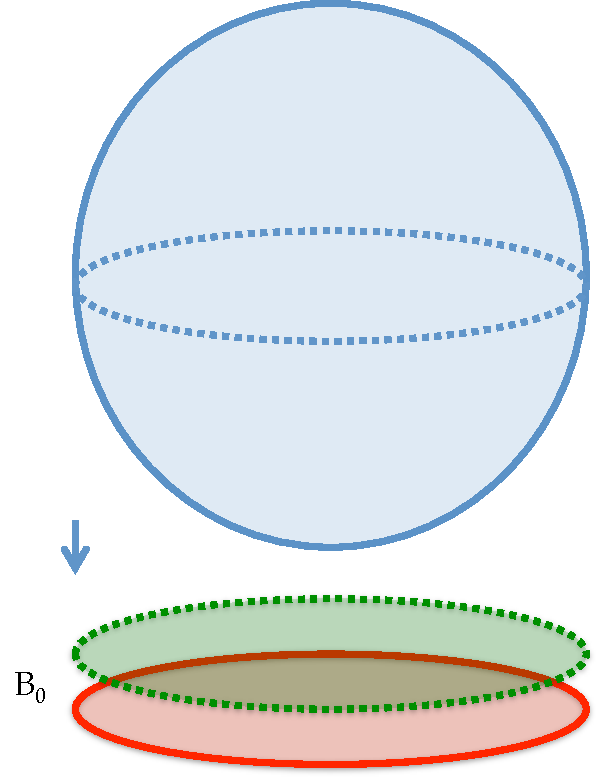
\includegraphics[width=.7\textwidth]{sphere_2dbc.pdf}
\end{center}
\caption{Two Dimensional Barcodes for the Sphere}
\label{fig:sphere2d_bc}
\end{figure}

\begin{ex}[Shadow of the Sphere]
	Consider the standard Euclidean sphere $S^2$ embedded in $\RR^3$. Let $f:S^2\to\RR^2$ be the projection onto the first two factors of $\RR^3$. The image $X=f(S^2)$ is the closed unit disk.

	One can use a multi-D analog of Corollary~\ref{cor:barcode_homology} to determine the homology of the two-sphere. 
	\[
		H_0(S^2)\cong H_0(X;\hF_0)\cong k \qquad H_1(S^2)\cong H_1(X;\hF_0)\cong 0 \qquad H_2(S^2)\cong H_2(X;\hF_0)\cong k
	\]
\end{ex}
